\hypertarget{stack_8h}{
\section{stack.h File Reference}
\label{stack_8h}\index{stack.h@{stack.h}}
}
This is brief description of this file. 


{\tt \#include \char`\"{}something.h\char`\"{}}\par
{\tt \#include $<$stdio.h$>$}\par


Include dependency graph for stack.h:\begin{figure}[H]
\begin{center}
\leavevmode
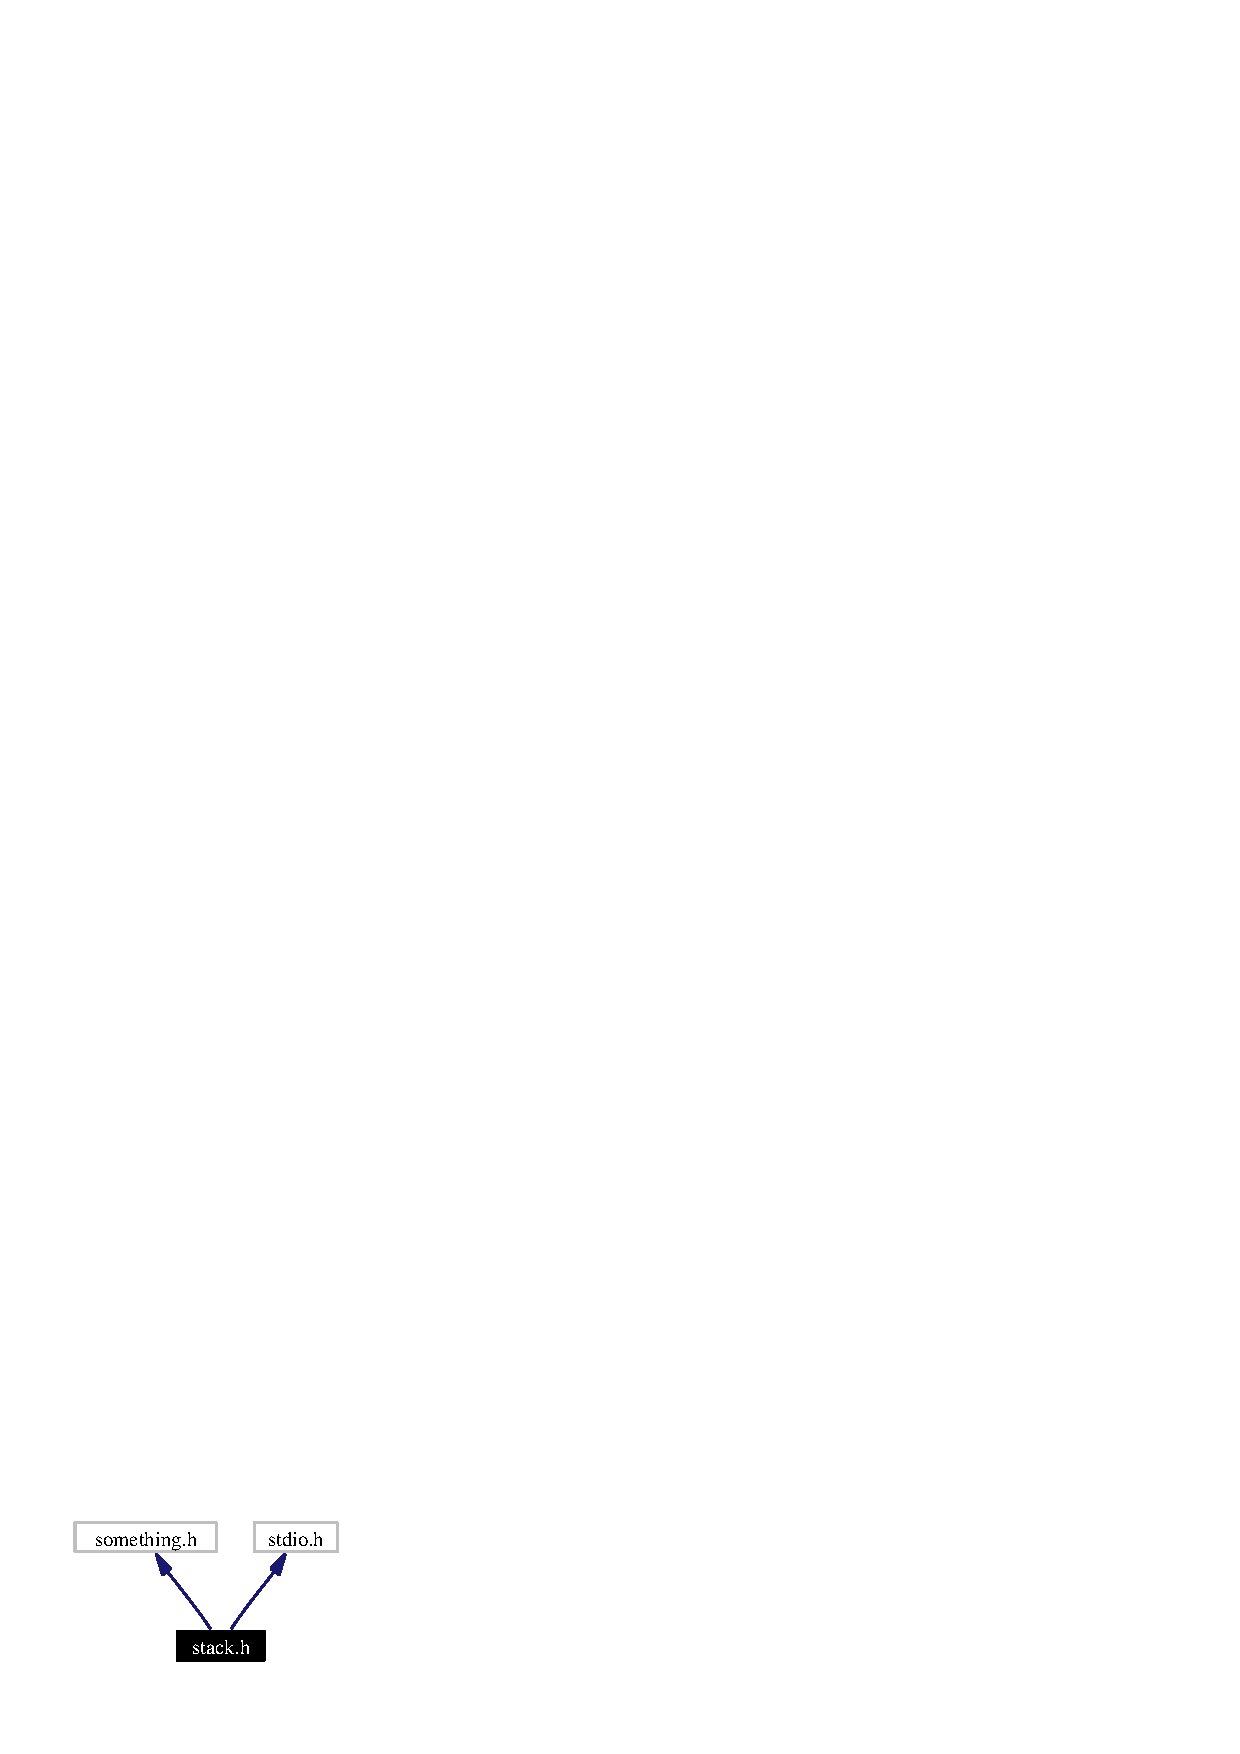
\includegraphics[width=81pt]{stack_8h__incl}
\end{center}
\end{figure}


This graph shows which files directly or indirectly include this file:\begin{figure}[H]
\begin{center}
\leavevmode
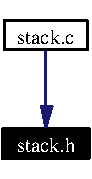
\includegraphics[width=39pt]{stack_8h__dep__incl}
\end{center}
\end{figure}
\subsection*{Data Structures}
\begin{CompactItemize}
\item 
struct \hyperlink{structstack}{stack}
\begin{CompactList}\small\item\em This is a stack struct.\item\end{CompactList}\end{CompactItemize}
\subsection*{Defines}
\begin{CompactItemize}
\item 
\#define \hyperlink{stack_8h_a0}{ENOMEM}\ -1
\item 
\hypertarget{stack_8h_a1}{
\index{EXAMPLE@{EXAMPLE}!stack.h@{stack.h}}\index{stack.h@{stack.h}!EXAMPLE@{EXAMPLE}}
\#define \hyperlink{stack_8h_a1}{EXAMPLE}\ -2}
\label{stack_8h_a1}

\begin{CompactList}\small\item\em you may also only have one line of comments\item\end{CompactList}\item 
\hypertarget{stack_8h_a2}{
\index{EXAMPLE2@{EXAMPLE2}!stack.h@{stack.h}}\index{stack.h@{stack.h}!EXAMPLE2@{EXAMPLE2}}
\#define \hyperlink{stack_8h_a2}{EXAMPLE2}\ -3}
\label{stack_8h_a2}

\begin{CompactList}\small\item\em This is how you put documentation after the fact.\item\end{CompactList}\end{CompactItemize}
\subsection*{Functions}
\begin{CompactItemize}
\item 
int \hyperlink{stack_8h_a3}{push} (\hyperlink{structstack}{stack} s, int val)
\begin{CompactList}\small\item\em This function is used to push stuff.\item\end{CompactList}\item 
int \hyperlink{group__stack_a1}{pop} (\hyperlink{structstack}{stack} s)
\begin{CompactList}\small\item\em This pops.\item\end{CompactList}\item 
int \hyperlink{stack_8h_a5}{get\_\-elem} (\hyperlink{structstack}{stack} s, int val)
\begin{CompactList}\small\item\em This gets an element.\item\end{CompactList}\item 
int \hyperlink{group__stack_a2}{top} (\hyperlink{structstack}{stack} s)
\begin{CompactList}\small\item\em Take a look at the top.\item\end{CompactList}\end{CompactItemize}


\subsection{Detailed Description}
This is brief description of this file.

 This is a slightly longer description of the file. Also note that the 'backslash'file command is needed or doxygen wont pull any declarations from the file \begin{Desc}
\item[Version: ]\par
a million \end{Desc}
\begin{Desc}
\item[Author: ]\par
someone without much to do , some other guy too \end{Desc}
\begin{Desc}
\item[Date: ]\par
1896-2430\end{Desc}


Definition in file \hyperlink{stack_8h-source}{stack.h}.

\subsection{Define Documentation}
\hypertarget{stack_8h_a0}{
\index{stack.h@{stack.h}!ENOMEM@{ENOMEM}}
\index{ENOMEM@{ENOMEM}!stack.h@{stack.h}}
\subsubsection[ENOMEM]{\setlength{\rightskip}{0pt plus 5cm}\#define ENOMEM\ -1}}
\label{stack_8h_a0}


This describes this define and what it is used for.  In this case it is used to say there is no memory.  These are automatically brief descriptions 

Definition at line 29 of file stack.h.

\subsection{Function Documentation}
\hypertarget{stack_8h_a5}{
\index{stack.h@{stack.h}!get_elem@{get\_\-elem}}
\index{get_elem@{get\_\-elem}!stack.h@{stack.h}}
\subsubsection[get\_\-elem]{\setlength{\rightskip}{0pt plus 5cm}int get\_\-elem (\hyperlink{structstack}{stack} {\em s}, int {\em val})}}
\label{stack_8h_a5}


This gets an element.

It is used to get stuff

\begin{Desc}
\item[\hyperlink{deprecated__deprecated000001}{Deprecated: }]\par
Dont use this anymore, for various reasons\end{Desc}
 \begin{Desc}
\item[Parameters: ]\par
\begin{description}
\item[{\em 
s}]stack to get item from \item[{\em 
i}]This is the index\end{description}
\end{Desc}
\begin{Desc}
\item[Returns: ]\par
\end{Desc}
\hypertarget{stack_8h_a3}{
\index{stack.h@{stack.h}!push@{push}}
\index{push@{push}!stack.h@{stack.h}}
\subsubsection[push]{\setlength{\rightskip}{0pt plus 5cm}int push (\hyperlink{structstack}{stack} {\em s}, int {\em val})}}
\label{stack_8h_a3}


This function is used to push stuff.

It puts stuff on the end.

\begin{Desc}
\item[\hyperlink{bug__bug000001}{Bug: }]\par
this function rules too much\end{Desc}
 \begin{Desc}
\item[Parameters: ]\par
\begin{description}
\item[{\em 
s}]This is the stack to push onto \item[{\em 
val}]This is the value to push\end{description}
\end{Desc}
\begin{Desc}
\item[Returns: ]\par
\begin{CompactItemize}
\item 
a non-negative value indicates success\item 
a negative return value indicates that the push was not successful\item 
The - creates a bullet list \end{CompactItemize}
\end{Desc}


Definition at line 13 of file stack.c.

References stack::end, and stack::stack.